\chapter{Changes in python script}
In order to make the measurements as described in the Introduction section, this time the value of the central barrier gate
is swept in a range that goes from $0.37$ V to $0.42$ V, taking 6 equally spaced values within this range:
\begin{lstlisting}[language=Python, label={init}, frame=single, framesep=8pt ]
    V_Barrier_Vec_2 = np.linspace(0.37,0.42, 6)
\end{lstlisting}
For each value of the central barrier gate, the program solves the non-linear Poisson equation and subsequently the Schrodinger equation, in order to obtain the energy levels of the system analyzed.
The workflow of the program consists of the following procedure:
\begin{itemize}
    \item Setting of the voltage values for all the required bias gates, including the one that will vary within a specific range.
    \item Definition of the materials, assigning to each region of the system their corresponding physical properties, as in the previous laboratories.
    \item At the end, execution of the solvers for the Poisson and Schrödinger equations for each possible value within the variation range.
\end{itemize}

What we obtain at the end are the first five energy eigenvalues given by the Schrödinger equation for each physical setup corresponding to the different values of the central barrier gate. After that, the program calculates the difference between the energy of the ground state and the energy of the first excited state ($E_1 - E_0$). This splitting represents the energy distance between the ground states of the two separate quantum dots for each value of the barrier.

\chapter{Python for the analysis of the results}

The data vector obtained from the previous script contains six pairs of data; for each voltage value of the central barrier gate, we computed the energy splitting between the first two energy levels of the system. 

At low bias, which corresponds to a high potential barrier, the two quantum dots are isolated from one another. Consequently, their first energy levels are nearly degenerate, so the delta is low. As the barrier height is reduced by varying the gate voltage, the dots begin to interact. This coupling causes the respective wavefunctions to overlap, which breaks the degeneracy and forces the two energy levels to split. 

According to the WKB (Wentzel-Kramers-Brillouin) approximation, this energy splitting follows an exponential growth as the barrier height decreases. While a detailed physical derivation is provided in the theoretical section of this work, the python script presented here aims to verify this behavior by fitting the six numerical data points with an exponential function, defined as follows:

\begin{lstlisting}[language=Python, caption={Exponential fit function and curve fitting procedure.}]
def exp_fun(x, a, b):
    # a: zero-voltage splitting pre-factor; b: tunneling sensitivity (related to m* and barrier width)
    return a * np.exp(b * x)

# Perform the exponential fit using scipy.optimize.curve_fit
param_opt, param_cov = curve_fit(exp_fun, x_data, y_data, p0=[y_data[0], 10])
\end{lstlisting}

Finally, the optimized fitting curve was plotted alongside the six numerical data points to evaluate the consistency and accuracy of the WKB approximation for this specific system configuration.

\begin{figure}[H]
    \centering
    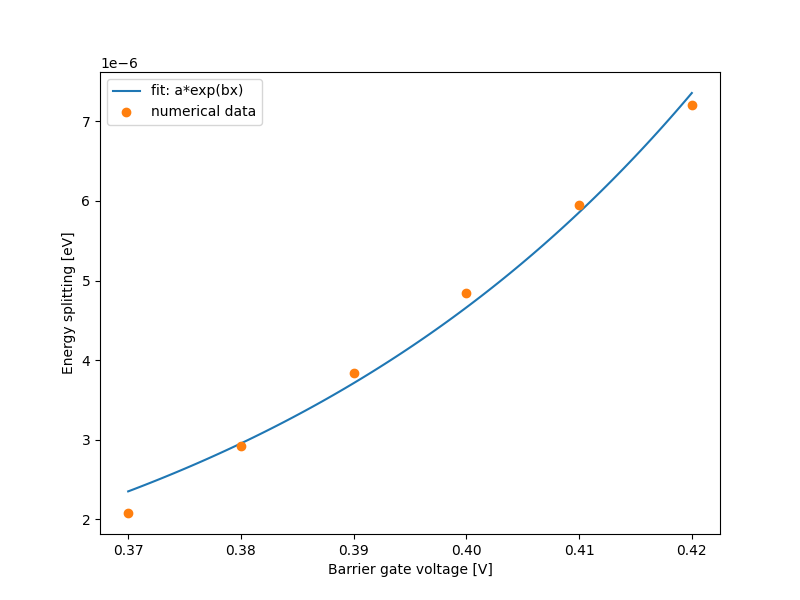
\includegraphics[width=0.8\textwidth]{leo_part/Plot_lab6.png} 
    \caption{Plot of the exponential fit alongside the six numerical data points, illustrating the increase in energy splitting as the central barrier height decreases.}
    \label{fig:plot}
\end{figure}

As shown in Fig.~\ref{fig:plot}, the exponential fit matches the numerical data reasonably well. However, despite the data points appearing somewhat linear, this is primarily due to the limited number of sampled points, which is insufficient to fully resolve the true exponential behavior over a wider range.